
\begin{figure}
	\centering
	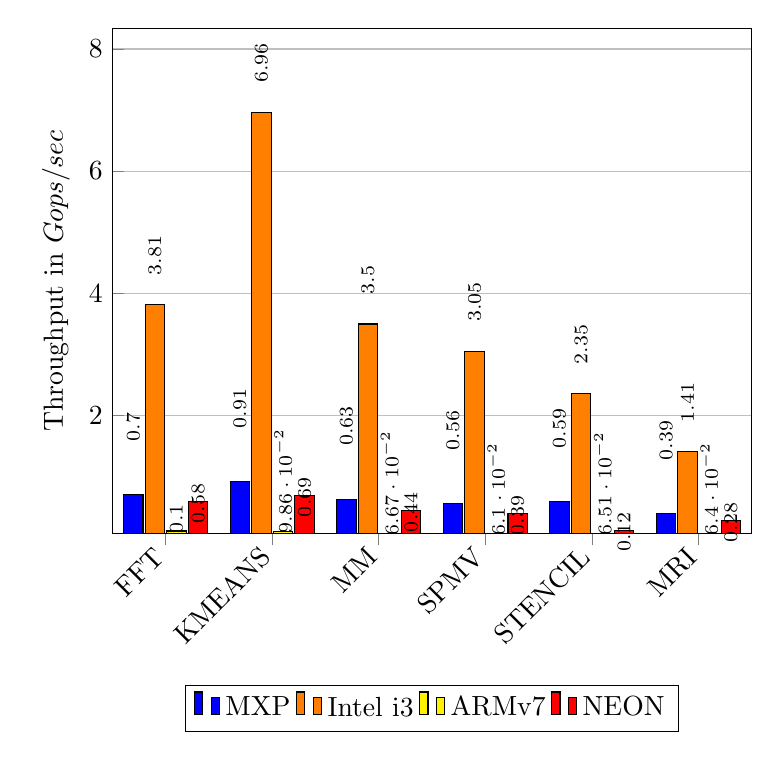
\begin{tikzpicture}
	\begin{axis}[
	width  = 0.8*\textwidth,
	height = 8cm,
	xtick pos=left,
    ytick pos=left,
%	major x tick style = transparent,
	x tick label style={rotate=45, anchor=east, align=right,text width=2cm},
	bar width=7pt,
	ymajorgrids = true,
	ylabel = {Throughput in $Gops/sec$},
	symbolic x coords={FFT,KMEANS,MM,SPMV,STENCIL,MRI},
	xtick = data,
	nodes near coords,
	ybar,
	every node near coord/.append style={rotate=90, anchor=west,font=\scriptsize, xshift=0.25cm},
	scaled y ticks = false,
	enlarge y limits={upper,value=0.2},
%	enlarge x limits=0.25,
	ybar=2*\pgflinewidth,
	legend cell align=left,
	legend style={
	at={(.5,-0.3)},
	anchor=north,
	legend columns=-1
	column sep=0.5ex
}
	]
	\addplot[draw=black,fill=blue,every node near coord/.append style={xshift=0.3cm}]
	coordinates {(FFT, 0.69951) (KMEANS,0.914) (MM,0.627) (SPMV,0.559) (STENCIL,0.589) (MRI,0.388)};
	
	\addplot[draw=black,fill=orange]
	coordinates  {(FFT,3.809) (KMEANS,6.96) (MM,3.495) (SPMV,3.05) (STENCIL,2.35) (MRI,1.406)};
	
	\addplot[draw=black,fill=yellow,every node near coord/.append style={xshift=-0.4cm}]
	coordinates  {(FFT,0.1042) (KMEANS,0.0986) (MM,0.0667) (SPMV,0.061) (STENCIL,0.0651) (MRI,0.064)};
	
	\addplot[draw=black,fill=red,every node near coord/.append style={xshift=-0.65cm}]
	coordinates {(FFT, 0.5833) (KMEANS,0.689) (MM,0.443) (SPMV,0.391) (STENCIL,0.1162) (MRI,0.277)};
	
	\legend{MXP,Intel i3,ARMv7,NEON}
	\end{axis}
	\end{tikzpicture}
	\caption{Byte(8-bits) level throughput(Gops/sec) for compute Kernels}
	\label{kernel:1}
\end{figure}

